\documentclass[12pt,a4paper]{article}
\usepackage[utf8]{vietnam}
\usepackage{amsmath,amssymb}
\usepackage{tabularx}
\usepackage{tikz}
\usepackage{xcolor}
\usepackage[top=0.6cm, bottom=0.6cm, left=0.6cm, right=0.6cm]{geometry}
\usepackage[dethi]{ex_test}

\SAOPTN{widthSA=2.6,heightSA=0.62}
\setlength{\parskip}{0pt}

% Dong ke cham mo chuan viet tay
\newcommand{\dongke}[1]{%
  \begingroup%
  \setlength{\parskip}{0pt}%
  \baselineskip=18.5pt%
  \vspace{1.0mm}%
  \foreach \i in {1,...,#1}{%
    \noindent{\color{gray!60}\dotfill}\par%
  }%
  \vspace{0.6mm}%
  \endgroup%
}

% Khu vuc bai lam chia 2 cot co vach ngan mo o giua
\newcommand{\dongkeHaiCot}[1]{%
  \par\vspace{0.5mm}%
  \noindent%
  \begin{minipage}[t]{0.485\linewidth}%
    \dongke{#1}%
  \end{minipage}%
  \hfill%
  {\color{gray!60}\vrule}%
  \hfill%
  \begin{minipage}[t]{0.485\linewidth}%
    \dongke{#1}%
  \end{minipage}%
}

% Dinh nghia o bai tap tu luan trong bang
\newcommand{\oBaiTap}[3][5]{%
  \vspace{1.0mm}%
  \noindent\textbf{#2} #3\par%
  \dongke{#1}%
}

\begin{document}
\pagestyle{empty}
% =============================================================================
% ========================= TOAN 7 TUAN 11 BUOI 02 - MA DE 101 =================
% ========================= TRANG 1/2 ==========================================
% =============================================================================
\noindent
\begin{tabularx}{\linewidth}{|X|c|}
\hline
\textbf{PHIẾU KIỂM TRA ĐỊNH KỲ TOÁN 7 - TUẦN 11 - BUỔI 02} & \textbf{Mã đề: 101 - Trang 1/2} \\
\hline
\end{tabularx}

\vspace{1.0mm}

\noindent
\begin{tabularx}{\linewidth}{|p{3.2cm}|X|}
\hline
\centering\textbf{ĐIỂM SỐ} & \centering\textbf{LỜI NHẬN XÉT CỦA THẦY CÔ} \tabularnewline
\hline
\rule{0pt}{1.8cm} & \tabularnewline
\hline
\end{tabularx}

\vspace{1.2mm}
\noindent\textbf{Câu 1 (0,25 điểm).} Trong $\Delta ABC$, cạnh kề hai góc $\widehat{B}$ và $\widehat{C}$ là: \shortans{BC}\par\vspace{3.0mm}
\noindent\textbf{Câu 2 (0,25 điểm).} Để $\Delta ABC = \Delta DEF$ (g.c.g) khi $\widehat{B}=\widehat{E}, BC=EF$, cần thêm: \shortans{\widehat{C} = \widehat{F}}\par\vspace{3.0mm}
\noindent\textbf{Câu 3 (0,25 điểm).} Cho $\Delta ABC, \Delta DEF$ vuông tại $A, D$, $BC=EF$. Cần thêm góc nhọn: \shortans{\widehat{B} = \widehat{E}}\par\vspace{3.0mm}
\noindent\textbf{Câu 4 (0,25 điểm).} Cho $\Delta ABC, \Delta DEF$ vuông tại $A, D$, $AB=DE$. Cần thêm góc nhọn: \shortans{\widehat{B} = \widehat{E}}\par\vspace{3.0mm}
\noindent\textbf{Câu 5 (0,25 điểm).} Cho $\Delta ABC = \Delta DEF$ (g.c.g), $\widehat{A}=70^\circ, \widehat{B}=45^\circ$. Khi đó $\widehat{F}$ bằng: \shortans{65^\circ}\par\vspace{3.0mm}
\noindent\textbf{Câu 6 (0,25 điểm).} Cho $\Delta ABC = \Delta MNP$ (g.c.g), biết $AC = 10\text{ cm}$. Độ dài cạnh $MP$ là: \shortans{10\text{ cm}}\par\vspace{3.0mm}
\noindent\textbf{Câu 7 (0,25 điểm).} Giá trị của biểu thức $3\sqrt{16} - 2\sqrt{25}$ bằng: \shortans{2}\par\vspace{3.0mm}
\noindent\textbf{Câu 8 (0,25 điểm).} Tìm số hữu tỉ $x < 0$, biết $|x + 1| = 3$: \shortans{x = -4}\par\vspace{3.0mm}
\noindent\textbf{Câu 9 (0,25 điểm).} Đo ra tàu qua $\Delta ABC = \Delta ABD$. Biết $AD = 62\text{ m}$. Khi đó $AC = $ \shortans{62\text{ m}}\par\vspace{3.0mm}
\noindent\textbf{Câu 10 (0,25 điểm).} Trong tam giác vuông, một góc nhọn bằng $35^\circ$ thì góc nhọn kia bằng: \shortans{55^\circ}\par\vspace{3.0mm}
\vspace{0.2mm}
\noindent\textbf{Câu 11 (3,0 điểm). Thực hiện phép tính (hợp lý nếu có thể):}
\vspace{0.6mm}

\noindent
\begin{tabularx}{\linewidth}{|X|X|}
\hline
\oBaiTap[5]{a) (0,5 điểm)}{$\dfrac{4}{15} - \dfrac{5}{12} + \dfrac{11}{15} - \dfrac{7}{12}$} & 
\oBaiTap[5]{b) (0,5 điểm)}{$\dfrac{3}{5} \cdot \dfrac{7}{11} + \dfrac{3}{5} \cdot \dfrac{4}{11} + \dfrac{2}{5}$} \\
\hline
\oBaiTap[5]{c) (0,5 điểm)}{$\left(-\dfrac{2}{3}\right)^2 : \dfrac{8}{9} + \left(-\dfrac{1}{2}\right)^3 \cdot 4$} & 
\oBaiTap[5]{d) (0,5 điểm)}{$\sqrt{\dfrac{49}{100}} - \left|-\dfrac{3}{10}\right| + \sqrt{0{,}36}$} \\
\hline
\oBaiTap[5]{e) (0,5 điểm)}{$\dfrac{2}{3} - \left[ \dfrac{1}{6} - \left(\dfrac{3}{4} - \dfrac{1}{2}\right) \right]$} & 
\oBaiTap[5]{f) (0,5 điểm)}{$\dfrac{9^3 \cdot 2^6}{6^5}$} \\
\hline
\end{tabularx}

\newpage
% =============================================================================
% ========================= TOAN 7 TUAN 11 BUOI 02 - MA DE 101 =================
% ========================= TRANG 2/2 ==========================================
% =============================================================================
\noindent
\begin{tabularx}{\linewidth}{|X|c|}
\hline
\textbf{TOÁN 7 - TUẦN 11 - BUỔI 02} & \textbf{Mã đề: 101 - Trang 2/2} \\
\hline
\end{tabularx}

\vspace{1.2mm}

\noindent\textbf{Câu 12 (2,0 điểm). Tìm số hữu tỉ $x$, biết:}
\vspace{0.6mm}

\noindent
\begin{tabularx}{\linewidth}{|X|X|}
\hline
\oBaiTap[5]{a) (0,5 điểm)}{$x - \dfrac{3}{4} = \dfrac{1}{8}$} & 
\oBaiTap[5]{b) (0,5 điểm)}{$\dfrac{3}{4}x + \dfrac{1}{3} = \dfrac{5}{6}$} \\
\hline
\oBaiTap[5]{c) (0,5 điểm)}{$\left(2x - \dfrac{1}{2}\right)^2 = \dfrac{9}{4}$} & 
\oBaiTap[5]{d) (0,5 điểm)}{$3\left|x - \dfrac{1}{2}\right| - \dfrac{1}{4} = \dfrac{5}{4}$} \\
\hline
\end{tabularx}

\vspace{1.2mm}

\noindent
\begin{tabularx}{\linewidth}{|X|}
\hline
\vspace{0.5mm}
\begin{minipage}[t]{0.68\linewidth}
\vspace{0pt}
\textbf{Câu 13 (2,0 điểm).} Cho đoạn thẳng $AB$ có trung điểm là $I$. Qua $I$ kẻ đường thẳng $xy$ (đường thẳng $xy$ không vuông góc với $AB$). Từ $A$ kẻ $AH \perp xy$ tại $H$, từ $B$ kẻ $BK \perp xy$ tại $K$.\par\vspace{0.4mm}
\textbf{a)} (1,0 điểm) Chứng minh rằng $\Delta AHI = \Delta BKI$ (cạnh huyền - góc nhọn).\par\vspace{0.4mm}
\textbf{b)} (1,0 điểm) Chứng minh rằng $AH = BK$ và $AH \parallel BK$.
\end{minipage}\hfill
\begin{minipage}[t]{0.30\linewidth}
\vspace{0pt}\centering
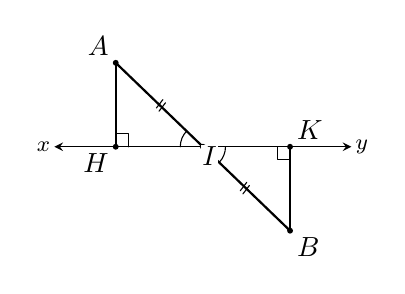
\begin{tikzpicture}[scale=0.82, >=stealth, line join=round, line cap=round]
  \coordinate (I) at (0, 0);
  \coordinate (X) at (-2.3, 0);
  \coordinate (Y) at (2.3, 0);
  \coordinate (A) at (-1.35, 1.3);
  \coordinate (B) at (1.35, -1.3);
  \coordinate (H) at (-1.35, 0);
  \coordinate (K) at (1.35, 0);

  \draw[<->] (X) node[left=-2pt] {{\footnotesize $x$}} -- (Y) node[right=-2pt] {{\footnotesize $y$}};

  \draw[thick] (A) -- (B);
  \draw[thick] (A) -- (H);
  \draw[thick] (B) -- (K);

  \draw (-1.35, 0.2) -- (-1.15, 0.2) -- (-1.15, 0);
  \draw (1.35, -0.2) -- (1.15, -0.2) -- (1.15, 0);

  \draw (-0.72, 0.6) -- (-0.62, 0.73);
  \draw (-0.68, 0.55) -- (-0.58, 0.68);
  \draw (0.62, -0.73) -- (0.72, -0.6);
  \draw (0.58, -0.68) -- (0.68, -0.55);

  \draw (-0.35, 0) arc (180:136:0.35);
  \draw (0.35, 0) arc (0:-44:0.35);

  \fill (I) circle (1.3pt) node[below right=-1pt, fill=white, inner sep=0.6pt] {{$I$}};
  \fill (A) circle (1.3pt) node[above left=-1pt] {{$A$}};
  \fill (B) circle (1.3pt) node[below right=-1pt] {{$B$}};
  \fill (H) circle (1.3pt) node[below left=-1pt] {{$H$}};
  \fill (K) circle (1.3pt) node[above right=-1pt] {{$K$}};
\end{tikzpicture}
\end{minipage}\par
\vspace{0.4mm}
\noindent\textit{Bài giải:}\dongkeHaiCot{10}
\\ \hline
\end{tabularx}

\vspace{1.2mm}

\noindent
\begin{tabularx}{\linewidth}{|X|}
\hline
\vspace{0.5mm}
\textbf{Câu 14 (0,5 điểm).} Tìm giá trị lớn nhất của biểu thức: $B = \dfrac{12}{|x - 3| + 4}$.\par
\vspace{0.4mm}
\noindent\textit{Bài giải:}\dongkeHaiCot{6}
\\ \hline
\end{tabularx}

\newpage
% =============================================================================
% ========================= TOAN 7 TUAN 11 BUOI 02 - MA DE 102 =================
% ========================= TRANG 1/2 ==========================================
% =============================================================================
\noindent
\begin{tabularx}{\linewidth}{|X|c|}
\hline
\textbf{PHIẾU KIỂM TRA ĐỊNH KỲ TOÁN 7 - TUẦN 11 - BUỔI 02} & \textbf{Mã đề: 102 - Trang 1/2} \\
\hline
\end{tabularx}

\vspace{1.0mm}

\noindent
\begin{tabularx}{\linewidth}{|p{3.2cm}|X|}
\hline
\centering\textbf{ĐIỂM SỐ} & \centering\textbf{LỜI NHẬN XÉT CỦA THẦY CÔ} \tabularnewline
\hline
\rule{0pt}{1.8cm} & \tabularnewline
\hline
\end{tabularx}

\vspace{1.2mm}
\noindent\textbf{Câu 1 (0,25 điểm).} Trong $\Delta MNP$, cạnh kề hai góc $\widehat{M}$ và $\widehat{P}$ là: \shortans{MP}\par\vspace{3.0mm}
\noindent\textbf{Câu 2 (0,25 điểm).} Để $\Delta MNP = \Delta QRS$ (g.c.g) khi $\widehat{M}=\widehat{Q}, MN=QR$, cần thêm: \shortans{\widehat{N} = \widehat{R}}\par\vspace{3.0mm}
\noindent\textbf{Câu 3 (0,25 điểm).} Cho $\Delta MNP, \Delta GHK$ vuông tại $M, G$, $NP=HK$. Cần thêm góc nhọn: \shortans{\widehat{N} = \widehat{H}}\par\vspace{3.0mm}
\noindent\textbf{Câu 4 (0,25 điểm).} Cho $\Delta MNP, \Delta DEF$ vuông tại $M, D$, $MP=DF$. Cần thêm góc nhọn: \shortans{\widehat{P} = \widehat{F}}\par\vspace{3.0mm}
\noindent\textbf{Câu 5 (0,25 điểm).} Cho $\Delta ABC = \Delta MNP$ (g.c.g), $\widehat{A}=65^\circ, \widehat{B}=55^\circ$. Khi đó $\widehat{P}$ bằng: \shortans{60^\circ}\par\vspace{3.0mm}
\noindent\textbf{Câu 6 (0,25 điểm).} Cho $\Delta ABC = \Delta MNP$ (g.c.g), biết $BC = 8\text{ cm}$. Độ dài cạnh $NP$ là: \shortans{8\text{ cm}}\par\vspace{3.0mm}
\noindent\textbf{Câu 7 (0,25 điểm).} Giá trị của biểu thức $2\sqrt{49} - 3\sqrt{16}$ bằng: \shortans{2}\par\vspace{3.0mm}
\noindent\textbf{Câu 8 (0,25 điểm).} Tìm số hữu tỉ $x < 0$, biết $|x + 2| = 5$: \shortans{x = -7}\par\vspace{3.0mm}
\noindent\textbf{Câu 9 (0,25 điểm).} Đo ra tàu qua $\Delta ABC = \Delta ABD$. Biết $AD = 75\text{ m}$. Khi đó $AC = $ \shortans{75\text{ m}}\par\vspace{3.0mm}
\noindent\textbf{Câu 10 (0,25 điểm).} Trong tam giác vuông, một góc nhọn bằng $40^\circ$ thì góc nhọn kia bằng: \shortans{50^\circ}\par\vspace{3.0mm}
\vspace{0.2mm}
\noindent\textbf{Câu 11 (3,0 điểm). Thực hiện phép tính (hợp lý nếu có thể):}
\vspace{0.6mm}

\noindent
\begin{tabularx}{\linewidth}{|X|X|}
\hline
\oBaiTap[5]{a) (0,5 điểm)}{$\dfrac{5}{18} - \dfrac{7}{16} + \dfrac{13}{18} - \dfrac{9}{16}$} & 
\oBaiTap[5]{b) (0,5 điểm)}{$\dfrac{4}{7} \cdot \dfrac{5}{13} + \dfrac{4}{7} \cdot \dfrac{8}{13} + \dfrac{3}{7}$} \\
\hline
\oBaiTap[5]{c) (0,5 điểm)}{$\left(-\dfrac{3}{4}\right)^2 : \dfrac{9}{8} + \left(-\dfrac{1}{3}\right)^2 \cdot (-9)$} & 
\oBaiTap[5]{d) (0,5 điểm)}{$\sqrt{\dfrac{81}{100}} - \left|-\dfrac{4}{10}\right| + \sqrt{0{,}25}$} \\
\hline
\oBaiTap[5]{e) (0,5 điểm)}{$\dfrac{3}{4} - \left[ \dfrac{1}{4} - \left(\dfrac{5}{6} - \dfrac{1}{3}\right) \right]$} & 
\oBaiTap[5]{f) (0,5 điểm)}{$\dfrac{8^3 \cdot 3^8}{6^7}$} \\
\hline
\end{tabularx}

\newpage
% =============================================================================
% ========================= TOAN 7 TUAN 11 BUOI 02 - MA DE 102 =================
% ========================= TRANG 2/2 ==========================================
% =============================================================================
\noindent
\begin{tabularx}{\linewidth}{|X|c|}
\hline
\textbf{TOÁN 7 - TUẦN 11 - BUỔI 02} & \textbf{Mã đề: 102 - Trang 2/2} \\
\hline
\end{tabularx}

\vspace{1.2mm}

\noindent\textbf{Câu 12 (2,0 điểm). Tìm số hữu tỉ $x$, biết:}
\vspace{0.6mm}

\noindent
\begin{tabularx}{\linewidth}{|X|X|}
\hline
\oBaiTap[5]{a) (0,5 điểm)}{$x - \dfrac{2}{3} = \dfrac{1}{6}$} & 
\oBaiTap[5]{b) (0,5 điểm)}{$\dfrac{2}{5}x + \dfrac{1}{2} = \dfrac{9}{10}$} \\
\hline
\oBaiTap[5]{c) (0,5 điểm)}{$\left(2x - \dfrac{1}{3}\right)^2 = \dfrac{25}{9}$} & 
\oBaiTap[5]{d) (0,5 điểm)}{$2\left|x - \dfrac{2}{3}\right| - \dfrac{1}{3} = \dfrac{5}{3}$} \\
\hline
\end{tabularx}

\vspace{1.2mm}

\noindent
\begin{tabularx}{\linewidth}{|X|}
\hline
\vspace{0.5mm}
\begin{minipage}[t]{0.68\linewidth}
\vspace{0pt}
\textbf{Câu 13 (2,0 điểm).} Cho đoạn thẳng $CD$ có trung điểm là $O$. Qua $O$ kẻ đường thẳng $mn$ (đường thẳng $mn$ không vuông góc với $CD$). Từ $C$ kẻ $CE \perp mn$ tại $E$, từ $D$ kẻ $DF \perp mn$ tại $F$.\par\vspace{0.4mm}
\textbf{a)} (1,0 điểm) Chứng minh rằng $\Delta CEO = \Delta DFO$ (cạnh huyền - góc nhọn).\par\vspace{0.4mm}
\textbf{b)} (1,0 điểm) Chứng minh rằng $CE = DF$ và $CE \parallel DF$.
\end{minipage}\hfill
\begin{minipage}[t]{0.30\linewidth}
\vspace{0pt}\centering
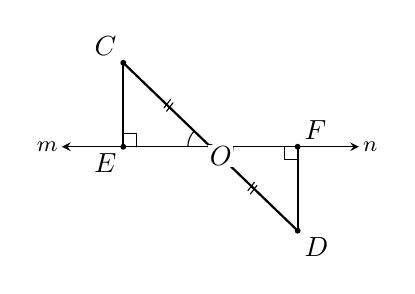
\begin{tikzpicture}[scale=0.82, >=stealth, line join=round, line cap=round]
  \coordinate (O) at (0, 0);
  \coordinate (M) at (-2.3, 0);
  \coordinate (N) at (2.3, 0);
  \coordinate (C) at (-1.35, 1.3);
  \coordinate (D) at (1.35, -1.3);
  \coordinate (E) at (-1.35, 0);
  \coordinate (F) at (1.35, 0);

  \draw[<->] (M) node[left=-2pt] {{\footnotesize $m$}} -- (N) node[right=-2pt] {{\footnotesize $n$}};

  \draw[thick] (C) -- (D);
  \draw[thick] (C) -- (E);
  \draw[thick] (D) -- (F);

  \draw (-1.35, 0.2) -- (-1.15, 0.2) -- (-1.15, 0);
  \draw (1.35, -0.2) -- (1.15, -0.2) -- (1.15, 0);

  \draw (-0.72, 0.6) -- (-0.62, 0.73);
  \draw (-0.68, 0.55) -- (-0.58, 0.68);
  \draw (0.62, -0.73) -- (0.72, -0.6);
  \draw (0.58, -0.68) -- (0.68, -0.55);

  \draw (-0.35, 0) arc (180:136:0.35);
  \draw (0.35, 0) arc (0:-44:0.35);

  \fill (O) circle (1.3pt) node[below right=-1pt, fill=white, inner sep=0.6pt] {{$O$}};
  \fill (C) circle (1.3pt) node[above left=-1pt] {{$C$}};
  \fill (D) circle (1.3pt) node[below right=-1pt] {{$D$}};
  \fill (E) circle (1.3pt) node[below left=-1pt] {{$E$}};
  \fill (F) circle (1.3pt) node[above right=-1pt] {{$F$}};
\end{tikzpicture}
\end{minipage}\par
\vspace{0.4mm}
\noindent\textit{Bài giải:}\dongkeHaiCot{10}
\\ \hline
\end{tabularx}

\vspace{1.2mm}

\noindent
\begin{tabularx}{\linewidth}{|X|}
\hline
\vspace{0.5mm}
\textbf{Câu 14 (0,5 điểm).} Tìm giá trị lớn nhất của biểu thức: $B = \dfrac{15}{|x - 2| + 5}$.\par
\vspace{0.4mm}
\noindent\textit{Bài giải:}\dongkeHaiCot{6}
\\ \hline
\end{tabularx}

\newpage
% =============================================================================
% ========================= TOAN 7 TUAN 11 BUOI 02 - MA DE 103 =================
% ========================= TRANG 1/2 ==========================================
% =============================================================================
\noindent
\begin{tabularx}{\linewidth}{|X|c|}
\hline
\textbf{PHIẾU KIỂM TRA ĐỊNH KỲ TOÁN 7 - TUẦN 11 - BUỔI 02} & \textbf{Mã đề: 103 - Trang 1/2} \\
\hline
\end{tabularx}

\vspace{1.0mm}

\noindent
\begin{tabularx}{\linewidth}{|p{3.2cm}|X|}
\hline
\centering\textbf{ĐIỂM SỐ} & \centering\textbf{LỜI NHẬN XÉT CỦA THẦY CÔ} \tabularnewline
\hline
\rule{0pt}{1.8cm} & \tabularnewline
\hline
\end{tabularx}

\vspace{1.2mm}
\noindent\textbf{Câu 1 (0,25 điểm).} Trong $\Delta DEF$, cạnh kề hai góc $\widehat{D}$ và $\widehat{E}$ là: \shortans{DE}\par\vspace{3.0mm}
\noindent\textbf{Câu 2 (0,25 điểm).} Để $\Delta ABC = \Delta MNP$ (g.c.g) khi $\widehat{A}=\widehat{M}, AC=MP$, cần thêm: \shortans{\widehat{C} = \widehat{P}}\par\vspace{3.0mm}
\noindent\textbf{Câu 3 (0,25 điểm).} Cho $\Delta ABC, \Delta MNP$ vuông tại $B, N$, $AC=MP$. Cần thêm góc nhọn: \shortans{\widehat{A} = \widehat{M}}\par\vspace{3.0mm}
\noindent\textbf{Câu 4 (0,25 điểm).} Cho $\Delta ABC, \Delta MNP$ vuông tại $B, N$, $BC=NP$. Cần thêm góc nhọn: \shortans{\widehat{C} = \widehat{P}}\par\vspace{3.0mm}
\noindent\textbf{Câu 5 (0,25 điểm).} Cho $\Delta DEF = \Delta GHK$ (g.c.g), $\widehat{D}=50^\circ, \widehat{E}=80^\circ$. Khi đó $\widehat{K}$ bằng: \shortans{50^\circ}\par\vspace{3.0mm}
\noindent\textbf{Câu 6 (0,25 điểm).} Cho $\Delta DEF = \Delta MNP$ (g.c.g), biết $DF = 8\text{ cm}$. Độ dài cạnh $MP$ là: \shortans{8\text{ cm}}\par\vspace{3.0mm}
\noindent\textbf{Câu 7 (0,25 điểm).} Giá trị của biểu thức $4\sqrt{25} - 2\sqrt{81}$ bằng: \shortans{2}\par\vspace{3.0mm}
\noindent\textbf{Câu 8 (0,25 điểm).} Tìm số hữu tỉ $x < 0$, biết $|x + 3| = 4$: \shortans{x = -7}\par\vspace{3.0mm}
\noindent\textbf{Câu 9 (0,25 điểm).} Đo ra tàu qua $\Delta ABC = \Delta ABD$. Biết $AD = 84\text{ m}$. Khi đó $AC = $ \shortans{84\text{ m}}\par\vspace{3.0mm}
\noindent\textbf{Câu 10 (0,25 điểm).} Trong tam giác vuông, một góc nhọn bằng $25^\circ$ thì góc nhọn kia bằng: \shortans{65^\circ}\par\vspace{3.0mm}
\vspace{0.2mm}
\noindent\textbf{Câu 11 (3,0 điểm). Thực hiện phép tính (hợp lý nếu có thể):}
\vspace{0.6mm}

\noindent
\begin{tabularx}{\linewidth}{|X|X|}
\hline
\oBaiTap[5]{a) (0,5 điểm)}{$\dfrac{3}{14} - \dfrac{5}{9} + \dfrac{11}{14} - \dfrac{4}{9}$} & 
\oBaiTap[5]{b) (0,5 điểm)}{$\dfrac{5}{8} \cdot \dfrac{4}{9} + \dfrac{5}{8} \cdot \dfrac{5}{9} + \dfrac{3}{8}$} \\
\hline
\oBaiTap[5]{c) (0,5 điểm)}{$\left(-\dfrac{1}{2}\right)^3 : \dfrac{1}{8} + \left(-\dfrac{2}{5}\right)^0$} & 
\oBaiTap[5]{d) (0,5 điểm)}{$\sqrt{\dfrac{64}{100}} - \left|-\dfrac{1}{10}\right| + \sqrt{0{,}09}$} \\
\hline
\oBaiTap[5]{e) (0,5 điểm)}{$\dfrac{5}{6} - \left[ \dfrac{1}{3} - \left(\dfrac{3}{4} - \dfrac{1}{4}\right) \right]$} & 
\oBaiTap[5]{f) (0,5 điểm)}{$\dfrac{25^2 \cdot 2^5}{10^4}$} \\
\hline
\end{tabularx}

\newpage
% =============================================================================
% ========================= TOAN 7 TUAN 11 BUOI 02 - MA DE 103 =================
% ========================= TRANG 2/2 ==========================================
% =============================================================================
\noindent
\begin{tabularx}{\linewidth}{|X|c|}
\hline
\textbf{TOÁN 7 - TUẦN 11 - BUỔI 02} & \textbf{Mã đề: 103 - Trang 2/2} \\
\hline
\end{tabularx}

\vspace{1.2mm}

\noindent\textbf{Câu 12 (2,0 điểm). Tìm số hữu tỉ $x$, biết:}
\vspace{0.6mm}

\noindent
\begin{tabularx}{\linewidth}{|X|X|}
\hline
\oBaiTap[5]{a) (0,5 điểm)}{$x + \dfrac{1}{4} = \dfrac{5}{8}$} & 
\oBaiTap[5]{b) (0,5 điểm)}{$\dfrac{4}{5}x - \dfrac{1}{2} = \dfrac{3}{10}$} \\
\hline
\oBaiTap[5]{c) (0,5 điểm)}{$\left(3x - \dfrac{1}{2}\right)^2 = \dfrac{25}{4}$} & 
\oBaiTap[5]{d) (0,5 điểm)}{$4\left|x - \dfrac{1}{3}\right| - \dfrac{2}{3} = \dfrac{10}{3}$} \\
\hline
\end{tabularx}

\vspace{1.2mm}

\noindent
\begin{tabularx}{\linewidth}{|X|}
\hline
\vspace{0.5mm}
\begin{minipage}[t]{0.68\linewidth}
\vspace{0pt}
\textbf{Câu 13 (2,0 điểm).} Cho đoạn thẳng $MN$ có trung điểm là $E$. Qua $E$ kẻ đường thẳng $pq$ (đường thẳng $pq$ không vuông góc với $MN$). Từ $M$ kẻ $MP \perp pq$ tại $P$, từ $N$ kẻ $NQ \perp pq$ tại $Q$.\par\vspace{0.4mm}
\textbf{a)} (1,0 điểm) Chứng minh rằng $\Delta MPE = \Delta NQE$ (cạnh huyền - góc nhọn).\par\vspace{0.4mm}
\textbf{b)} (1,0 điểm) Chứng minh rằng $MP = NQ$ và $MP \parallel NQ$.
\end{minipage}\hfill
\begin{minipage}[t]{0.30\linewidth}
\vspace{0pt}\centering
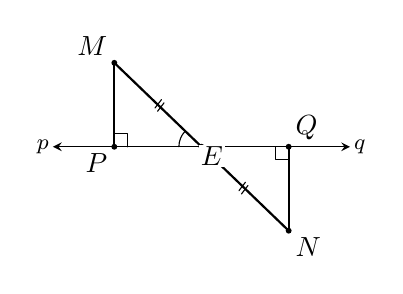
\begin{tikzpicture}[scale=0.82, >=stealth, line join=round, line cap=round]
  \coordinate (E) at (0, 0);
  \coordinate (P_axis) at (-2.3, 0);
  \coordinate (Q_axis) at (2.3, 0);
  \coordinate (M) at (-1.35, 1.3);
  \coordinate (N) at (1.35, -1.3);
  \coordinate (P) at (-1.35, 0);
  \coordinate (Q) at (1.35, 0);

  \draw[<->] (P_axis) node[left=-2pt] {{\footnotesize $p$}} -- (Q_axis) node[right=-2pt] {{\footnotesize $q$}};

  \draw[thick] (M) -- (N);
  \draw[thick] (M) -- (P);
  \draw[thick] (N) -- (Q);

  \draw (-1.35, 0.2) -- (-1.15, 0.2) -- (-1.15, 0);
  \draw (1.35, -0.2) -- (1.15, -0.2) -- (1.15, 0);

  \draw (-0.72, 0.6) -- (-0.62, 0.73);
  \draw (-0.68, 0.55) -- (-0.58, 0.68);
  \draw (0.62, -0.73) -- (0.72, -0.6);
  \draw (0.58, -0.68) -- (0.68, -0.55);

  \draw (-0.35, 0) arc (180:136:0.35);
  \draw (0.35, 0) arc (0:-44:0.35);

  \fill (E) circle (1.3pt) node[below right=-1pt, fill=white, inner sep=0.6pt] {{$E$}};
  \fill (M) circle (1.3pt) node[above left=-1pt] {{$M$}};
  \fill (N) circle (1.3pt) node[below right=-1pt] {{$N$}};
  \fill (P) circle (1.3pt) node[below left=-1pt] {{$P$}};
  \fill (Q) circle (1.3pt) node[above right=-1pt] {{$Q$}};
\end{tikzpicture}
\end{minipage}\par
\vspace{0.4mm}
\noindent\textit{Bài giải:}\dongkeHaiCot{10}
\\ \hline
\end{tabularx}

\vspace{1.2mm}

\noindent
\begin{tabularx}{\linewidth}{|X|}
\hline
\vspace{0.5mm}
\textbf{Câu 14 (0,5 điểm).} Tìm giá trị lớn nhất của biểu thức: $B = \dfrac{18}{|x - 5| + 6}$.\par
\vspace{0.4mm}
\noindent\textit{Bài giải:}\dongkeHaiCot{6}
\\ \hline
\end{tabularx}

\newpage
% =============================================================================
% ========================= TOAN 7 TUAN 11 BUOI 02 - MA DE 104 =================
% ========================= TRANG 1/2 ==========================================
% =============================================================================
\noindent
\begin{tabularx}{\linewidth}{|X|c|}
\hline
\textbf{PHIẾU KIỂM TRA ĐỊNH KỲ TOÁN 7 - TUẦN 11 - BUỔI 02} & \textbf{Mã đề: 104 - Trang 1/2} \\
\hline
\end{tabularx}

\vspace{1.0mm}

\noindent
\begin{tabularx}{\linewidth}{|p{3.2cm}|X|}
\hline
\centering\textbf{ĐIỂM SỐ} & \centering\textbf{LỜI NHẬN XÉT CỦA THẦY CÔ} \tabularnewline
\hline
\rule{0pt}{1.8cm} & \tabularnewline
\hline
\end{tabularx}

\vspace{1.2mm}
\noindent\textbf{Câu 1 (0,25 điểm).} Trong $\Delta HIK$, cạnh kề hai góc $\widehat{I}$ và $\widehat{K}$ là: \shortans{IK}\par\vspace{3.0mm}
\noindent\textbf{Câu 2 (0,25 điểm).} Để $\Delta DEF = \Delta HIK$ (g.c.g) khi $\widehat{E}=\widehat{I}, EF=IK$, cần thêm: \shortans{\widehat{F} = \widehat{K}}\par\vspace{3.0mm}
\noindent\textbf{Câu 3 (0,25 điểm).} Cho $\Delta DEF, \Delta HIK$ vuông tại $E, I$, $DF=HK$. Cần thêm góc nhọn: \shortans{\widehat{D} = \widehat{H}}\par\vspace{3.0mm}
\noindent\textbf{Câu 4 (0,25 điểm).} Cho $\Delta DEF, \Delta HIK$ vuông tại $E, I$, $DE=HI$. Cần thêm góc nhọn: \shortans{\widehat{D} = \widehat{H}}\par\vspace{3.0mm}
\noindent\textbf{Câu 5 (0,25 điểm).} Cho $\Delta ABC = \Delta DEF$ (g.c.g), $\widehat{A}=75^\circ, \widehat{B}=35^\circ$. Khi đó $\widehat{F}$ bằng: \shortans{70^\circ}\par\vspace{3.0mm}
\noindent\textbf{Câu 6 (0,25 điểm).} Cho $\Delta ABC = \Delta HIK$ (g.c.g), biết $AB = 6\text{ cm}$. Độ dài cạnh $HI$ là: \shortans{6\text{ cm}}\par\vspace{3.0mm}
\noindent\textbf{Câu 7 (0,25 điểm).} Giá trị của biểu thức $5\sqrt{9} - 2\sqrt{36}$ bằng: \shortans{3}\par\vspace{3.0mm}
\noindent\textbf{Câu 8 (0,25 điểm).} Tìm số hữu tỉ $x < 0$, biết $|x + 1| = 5$: \shortans{x = -6}\par\vspace{3.0mm}
\noindent\textbf{Câu 9 (0,25 điểm).} Đo ra tàu qua $\Delta ABC = \Delta ABD$. Biết $AD = 96\text{ m}$. Khi đó $AC = $ \shortans{96\text{ m}}\par\vspace{3.0mm}
\noindent\textbf{Câu 10 (0,25 điểm).} Trong tam giác vuông, một góc nhọn bằng $48^\circ$ thì góc nhọn kia bằng: \shortans{42^\circ}\par\vspace{3.0mm}
\vspace{0.2mm}
\noindent\textbf{Câu 11 (3,0 điểm). Thực hiện phép tính (hợp lý nếu có thể):}
\vspace{0.6mm}

\noindent
\begin{tabularx}{\linewidth}{|X|X|}
\hline
\oBaiTap[5]{a) (0,5 điểm)}{$\dfrac{6}{19} - \dfrac{3}{8} + \dfrac{13}{19} - \dfrac{5}{8}$} & 
\oBaiTap[5]{b) (0,5 điểm)}{$\dfrac{2}{9} \cdot \dfrac{7}{15} + \dfrac{2}{9} \cdot \dfrac{8}{15} + \dfrac{7}{9}$} \\
\hline
\oBaiTap[5]{c) (0,5 điểm)}{$\left(-\dfrac{1}{3}\right)^3 \cdot 27 + \left(\dfrac{4}{9}\right)^0$} & 
\oBaiTap[5]{d) (0,5 điểm)}{$\sqrt{\dfrac{121}{100}} - \left|-\dfrac{5}{10}\right| + \sqrt{0{,}16}$} \\
\hline
\oBaiTap[5]{e) (0,5 điểm)}{$\dfrac{4}{5} - \left[ \dfrac{1}{5} - \left(\dfrac{7}{10} - \dfrac{3}{10}\right) \right]$} & 
\oBaiTap[5]{f) (0,5 điểm)}{$\dfrac{27^3 \cdot 2^8}{6^8}$} \\
\hline
\end{tabularx}

\newpage
% =============================================================================
% ========================= TOAN 7 TUAN 11 BUOI 02 - MA DE 104 =================
% ========================= TRANG 2/2 ==========================================
% =============================================================================
\noindent
\begin{tabularx}{\linewidth}{|X|c|}
\hline
\textbf{TOÁN 7 - TUẦN 11 - BUỔI 02} & \textbf{Mã đề: 104 - Trang 2/2} \\
\hline
\end{tabularx}

\vspace{1.2mm}

\noindent\textbf{Câu 12 (2,0 điểm). Tìm số hữu tỉ $x$, biết:}
\vspace{0.6mm}

\noindent
\begin{tabularx}{\linewidth}{|X|X|}
\hline
\oBaiTap[5]{a) (0,5 điểm)}{$x + \dfrac{2}{5} = \dfrac{9}{10}$} & 
\oBaiTap[5]{b) (0,5 điểm)}{$\dfrac{5}{6}x - \dfrac{1}{4} = \dfrac{7}{12}$} \\
\hline
\oBaiTap[5]{c) (0,5 điểm)}{$\left(2x + \dfrac{1}{4}\right)^2 = \dfrac{49}{16}$} & 
\oBaiTap[5]{d) (0,5 điểm)}{$2\left|x - \dfrac{3}{4}\right| - \dfrac{1}{2} = \dfrac{3}{2}$} \\
\hline
\end{tabularx}

\vspace{1.2mm}

\noindent
\begin{tabularx}{\linewidth}{|X|}
\hline
\vspace{0.5mm}
\begin{minipage}[t]{0.68\linewidth}
\vspace{0pt}
\textbf{Câu 13 (2,0 điểm).} Cho đoạn thẳng $EF$ có trung điểm là $K$. Qua $K$ kẻ đường thẳng $uv$ (đường thẳng $uv$ không vuông góc với $EF$). Từ $E$ kẻ $EG \perp uv$ tại $G$, từ $F$ kẻ $FH \perp uv$ tại $H$.\par\vspace{0.4mm}
\textbf{a)} (1,0 điểm) Chứng minh rằng $\Delta EGK = \Delta FHK$ (cạnh huyền - góc nhọn).\par\vspace{0.4mm}
\textbf{b)} (1,0 điểm) Chứng minh rằng $EG = FH$ và $EG \parallel FH$.
\end{minipage}\hfill
\begin{minipage}[t]{0.30\linewidth}
\vspace{0pt}\centering
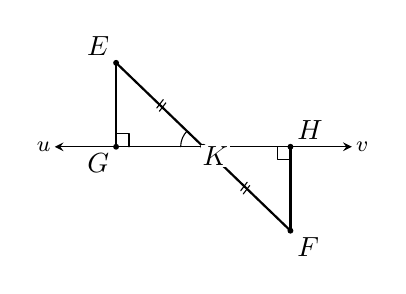
\begin{tikzpicture}[scale=0.82, >=stealth, line join=round, line cap=round]
  \coordinate (K) at (0, 0);
  \coordinate (U) at (-2.3, 0);
  \coordinate (V) at (2.3, 0);
  \coordinate (E) at (-1.35, 1.3);
  \coordinate (F) at (1.35, -1.3);
  \coordinate (G) at (-1.35, 0);
  \coordinate (H) at (1.35, 0);

  \draw[<->] (U) node[left=-2pt] {{\footnotesize $u$}} -- (V) node[right=-2pt] {{\footnotesize $v$}};

  \draw[thick] (E) -- (F);
  \draw[thick] (E) -- (G);
  \draw[thick] (F) -- (H);

  \draw (-1.35, 0.2) -- (-1.15, 0.2) -- (-1.15, 0);
  \draw (1.35, -0.2) -- (1.15, -0.2) -- (1.15, 0);

  \draw (-0.72, 0.6) -- (-0.62, 0.73);
  \draw (-0.68, 0.55) -- (-0.58, 0.68);
  \draw (0.62, -0.73) -- (0.72, -0.6);
  \draw (0.58, -0.68) -- (0.68, -0.55);

  \draw (-0.35, 0) arc (180:136:0.35);
  \draw (0.35, 0) arc (0:-44:0.35);

  \fill (K) circle (1.3pt) node[below right=-1pt, fill=white, inner sep=0.6pt] {{$K$}};
  \fill (E) circle (1.3pt) node[above left=-1pt] {{$E$}};
  \fill (F) circle (1.3pt) node[below right=-1pt] {{$F$}};
  \fill (G) circle (1.3pt) node[below left=-1pt] {{$G$}};
  \fill (H) circle (1.3pt) node[above right=-1pt] {{$H$}};
\end{tikzpicture}
\end{minipage}\par
\vspace{0.4mm}
\noindent\textit{Bài giải:}\dongkeHaiCot{10}
\\ \hline
\end{tabularx}

\vspace{1.2mm}

\noindent
\begin{tabularx}{\linewidth}{|X|}
\hline
\vspace{0.5mm}
\textbf{Câu 14 (0,5 điểm).} Tìm giá trị lớn nhất của biểu thức: $B = \dfrac{20}{|x - 1| + 4}$.\par
\vspace{0.4mm}
\noindent\textit{Bài giải:}\dongkeHaiCot{6}
\\ \hline
\end{tabularx}
\end{document}
